\chapter{MIPS Machine Language}

\section{The machine model}

CS 241 uses a simplified 32-bit MIPS machine:
\begin{itemize}
  \item 32 general-purpose registers \code{\$0}--\code{\$31}, each one word.
  \item Two special registers \code{hi} and \code{lo} that receive the results of multiplication
        and division.
  \item A program counter \code{PC} and an instruction register \code{IR} (not directly accessible).
  \item Byte-addressed RAM; all loads and stores are whole, word-aligned words.
\end{itemize}

\subsection{Register conventions}
Most registers are general purpose, but a few have fixed roles in CS 241:

\begin{center}
\begin{tabular}{lp{10cm}}
\toprule
register & role \\
\midrule
\code{\$0} & always 0; writes to it are discarded \\
\code{\$1}, \code{\$2} & inputs from the loader (\code{mips.twoints}, \code{mips.array}) \\
\code{\$3} & by convention the return value of the program / of procedures \\
\code{\$29} & frame pointer (used later by our WLP4 compiler) \\
\code{\$30} & stack pointer; initialised by the loader to the end of usable memory \\
\code{\$31} & return address; on start it holds the address that returns control to the loader \\
\bottomrule
\end{tabular}
\end{center}

\begin{important}[Ending a program]
A program is started like a procedure call: the loader sets \code{\$31} to a special return
address and jumps to address 0. The program terminates by executing \code{jr \$31}. If you
overwrite \code{\$31} (e.g.\ with \code{jalr}) you must save and restore it first.
\end{important}

\section{The instruction set}

Every instruction is exactly one 32-bit word. The CS 241 subset contains 18 instructions
plus the \code{.word} directive. Notation: $\$d, \$s, \$t$ are registers, $i$ is a 16-bit
immediate.

\begin{center}
\small
\begin{tabular}{lll}
\toprule
instruction & assembly & meaning \\
\midrule
add   & \code{add \$d, \$s, \$t} & $\$d \gets \$s + \$t$ \\
sub   & \code{sub \$d, \$s, \$t} & $\$d \gets \$s - \$t$ \\
mult  & \code{mult \$s, \$t}     & $\mathit{hi}{:}\mathit{lo} \gets \$s \times \$t$ (signed) \\
multu & \code{multu \$s, \$t}    & $\mathit{hi}{:}\mathit{lo} \gets \$s \times \$t$ (unsigned) \\
div   & \code{div \$s, \$t}      & $\mathit{lo} \gets \$s / \$t,\ \mathit{hi} \gets \$s \bmod \$t$ (signed) \\
divu  & \code{divu \$s, \$t}     & same, unsigned \\
mfhi  & \code{mfhi \$d}          & $\$d \gets \mathit{hi}$ \\
mflo  & \code{mflo \$d}          & $\$d \gets \mathit{lo}$ \\
lis   & \code{lis \$d}           & $\$d \gets \mathrm{MEM}[PC];\ PC \gets PC+4$ \\
lw    & \code{lw \$t, i(\$s)}    & $\$t \gets \mathrm{MEM}[\$s + i]$ \\
sw    & \code{sw \$t, i(\$s)}    & $\mathrm{MEM}[\$s + i] \gets \$t$ \\
slt   & \code{slt \$d, \$s, \$t} & $\$d \gets (\$s < \$t)\ ?\ 1 : 0$ (signed) \\
sltu  & \code{sltu \$d, \$s, \$t}& same, unsigned \\
beq   & \code{beq \$s, \$t, i}   & if $\$s = \$t$ then $PC \gets PC + 4i$ \\
bne   & \code{bne \$s, \$t, i}   & if $\$s \ne \$t$ then $PC \gets PC + 4i$ \\
jr    & \code{jr \$s}            & $PC \gets \$s$ \\
jalr  & \code{jalr \$s}          & $\mathit{tmp} \gets \$s;\ \$31 \gets PC;\ PC \gets \mathit{tmp}$ \\
.word & \code{.word i}           & a literal 32-bit word $i$ (not an instruction) \\
\bottomrule
\end{tabular}
\end{center}

Remarks:
\begin{itemize}
  \item In \code{beq}/\code{bne} the PC has \emph{already} been incremented, so the offset
        $i$ counts words relative to the instruction after the branch. $i = 0$ is a no-op;
        $i=-1$ is an infinite loop.
  \item \code{lis} (``load immediate and skip'') is a CS 241 invention: it loads the
        \emph{next word} of the program into $\$d$ and skips over it. It is always followed by
        a \code{.word}. This is how we get arbitrary 32-bit constants into registers.
  \item \code{mult} produces a 64-bit product; the high word goes to \code{hi}, low to \code{lo}.
        For small numbers you only need \code{mflo}.
  \item \code{div} rounds toward zero; the remainder has the sign of the dividend.
  \item \code{jalr} reads $\$s$ before writing \code{\$31}, so \code{jalr \$31} is well defined.
\end{itemize}

\section{Instruction encodings}

There are two formats used by our subset.

\paragraph{Register format (R-type).} Opcode 0, operation selected by the low 6 bits
(the \emph{function} field):
\begin{center}
\begin{tabular}{|c|c|c|c|c|c|}
\hline
\code{000000} & sssss & ttttt & ddddd & \code{00000} & ffffff \\
\hline
6 bits & 5 & 5 & 5 & 5 & 6 \\
\hline
\end{tabular}
\end{center}

\paragraph{Immediate format (I-type).} A 6-bit opcode, two registers, a 16-bit two's
complement immediate:
\begin{center}
\begin{tabular}{|c|c|c|c|}
\hline
oooooo & sssss & ttttt & iiii iiii iiii iiii \\
\hline
6 bits & 5 & 5 & 16 \\
\hline
\end{tabular}
\end{center}

\begin{center}
\small
\begin{tabular}{llll}
\toprule
instruction & fields used & opcode / funct & 32-bit pattern \\
\midrule
add   & s,t,d & funct \code{0x20} & \code{0000 00ss ssst tttt dddd d000 0010 0000} \\
sub   & s,t,d & funct \code{0x22} & \code{0000 00ss ssst tttt dddd d000 0010 0010} \\
mult  & s,t   & funct \code{0x18} & \code{0000 00ss ssst tttt 0000 0000 0001 1000} \\
multu & s,t   & funct \code{0x19} & \code{0000 00ss ssst tttt 0000 0000 0001 1001} \\
div   & s,t   & funct \code{0x1a} & \code{0000 00ss ssst tttt 0000 0000 0001 1010} \\
divu  & s,t   & funct \code{0x1b} & \code{0000 00ss ssst tttt 0000 0000 0001 1011} \\
mfhi  & d     & funct \code{0x10} & \code{0000 0000 0000 0000 dddd d000 0001 0000} \\
mflo  & d     & funct \code{0x12} & \code{0000 0000 0000 0000 dddd d000 0001 0010} \\
lis   & d     & funct \code{0x14} & \code{0000 0000 0000 0000 dddd d000 0001 0100} \\
slt   & s,t,d & funct \code{0x2a} & \code{0000 00ss ssst tttt dddd d000 0010 1010} \\
sltu  & s,t,d & funct \code{0x2b} & \code{0000 00ss ssst tttt dddd d000 0010 1011} \\
jr    & s     & funct \code{0x08} & \code{0000 00ss sss0 0000 0000 0000 0000 1000} \\
jalr  & s     & funct \code{0x09} & \code{0000 00ss sss0 0000 0000 0000 0000 1001} \\
lw    & s,t,i & op \code{0x23}    & \code{1000 11ss ssst tttt iiii iiii iiii iiii} \\
sw    & s,t,i & op \code{0x2b}    & \code{1010 11ss ssst tttt iiii iiii iiii iiii} \\
beq   & s,t,i & op \code{0x04}    & \code{0001 00ss ssst tttt iiii iiii iiii iiii} \\
bne   & s,t,i & op \code{0x05}    & \code{0001 01ss ssst tttt iiii iiii iiii iiii} \\
\bottomrule
\end{tabular}
\end{center}

\begin{important}[Field order trap]
In assembly, \code{add \$d, \$s, \$t} lists the destination first, but in the encoding $d$
comes \emph{after} $s$ and $t$. Similarly \code{lw \$t, i(\$s)}: the base register $s$ is
encoded first.
\end{important}

\begin{example}[Encoding \code{add \$3, \$1, \$2}]
$s=1=00001$, $t=2=00010$, $d=3=00011$, funct $=100000$:
\begin{align*}
&\mathtt{000000\,00001\,00010\,00011\,00000\,100000}\\
&= \mathtt{0000\,0000\,0010\,0010\,0001\,1000\,0010\,0000} = \mathtt{0x00221820}.
\end{align*}
\end{example}

\begin{example}[Encoding \code{beq \$1, \$0, -3}]
op $=000100$, $s=00001$, $t=00000$, $i = -3 = \mathtt{0xfffd}$ (16-bit two's complement):
\[
\mathtt{0001\,0000\,0010\,0000\,1111\,1111\,1111\,1101} = \mathtt{0x1020fffd}.
\]
\end{example}

\begin{example}[Decoding \code{0x8fc3fffc}]
Binary: \code{100011 11110 00011 1111111111111100}. Opcode \code{0x23} is \code{lw};
$s=30$, $t=3$, $i = \mathtt{0xfffc} = -4$. So the instruction is \code{lw \$3, -4(\$30)}.
\end{example}

The two encodings worked above, drawn as bit fields (bit numbers on top, 31 at the left):
\begin{center}
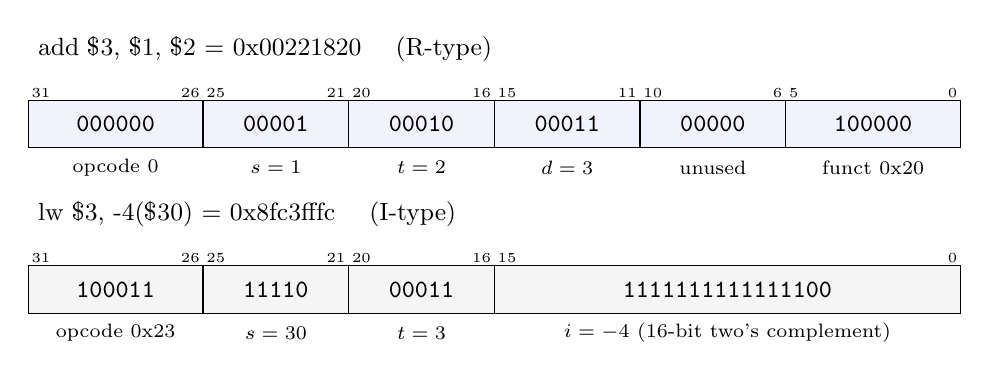
\begin{tikzpicture}[x=0.37cm,y=1cm,font=\small]
  \node[anchor=west] at (0,1.25) {\code{add \$3, \$1, \$2} $=$ \code{0x00221820} \quad (R-type)};
  \foreach \hi/\lo/\v/\f in {31/26/000000/opcode 0,25/21/00001/$s=1$,20/16/00010/$t=2$,15/11/00011/$d=3$,10/6/00000/unused,5/0/100000/funct \code{0x20}} {
    \draw[fill=blue!5] ({31-\hi},0) rectangle ({32-\lo},0.6);
    \node[font=\ttfamily\small] at ({(63-\hi-\lo)/2},0.3) {\v};
    \node[font=\scriptsize] at ({(63-\hi-\lo)/2},-0.25) {\f};
    \node[font=\tiny,anchor=south west,inner sep=1pt] at ({31-\hi},0.6) {\hi};
    \node[font=\tiny,anchor=south east,inner sep=1pt] at ({32-\lo},0.6) {\lo};
  }
  \begin{scope}[yshift=-2.1cm]
  \node[anchor=west] at (0,1.25) {\code{lw \$3, -4(\$30)} $=$ \code{0x8fc3fffc} \quad (I-type)};
  \foreach \hi/\lo/\v/\f in {31/26/100011/opcode \code{0x23},25/21/11110/$s=30$,20/16/00011/$t=3$,15/0/1111111111111100/$i=-4$ (16-bit two's complement)} {
    \draw[fill=gray!8] ({31-\hi},0) rectangle ({32-\lo},0.6);
    \node[font=\ttfamily\small] at ({(63-\hi-\lo)/2},0.3) {\v};
    \node[font=\scriptsize] at ({(63-\hi-\lo)/2},-0.25) {\f};
    \node[font=\tiny,anchor=south west,inner sep=1pt] at ({31-\hi},0.6) {\hi};
    \node[font=\tiny,anchor=south east,inner sep=1pt] at ({32-\lo},0.6) {\lo};
  }
  \end{scope}
\end{tikzpicture}
\end{center}

In code, encoding is done with shifts and masks; masking the immediate with
\code{0xffff} is essential so a negative immediate does not smear sign bits over the other
fields:
\begin{lstlisting}[style=cpp]
uint32_t encodeI(int op, int s, int t, int i) {
    return (op << 26) | (s << 21) | (t << 16) | (i & 0xffff);
}
uint32_t encodeR(int s, int t, int d, int funct) {
    return (s << 21) | (t << 16) | (d << 11) | funct;
}
\end{lstlisting}

\section{Loader conventions: \code{mips.twoints} and \code{mips.array}}

The course provides two front-ends that load a machine-code program at address 0 and run it.

\begin{description}
  \item[\code{mips.twoints}] prompts for two integers and places them in \code{\$1} and
        \code{\$2}.
  \item[\code{mips.array}] prompts for an array length and elements, stores the array
        somewhere in memory, and puts its \emph{address} in \code{\$1} and its \emph{length}
        in \code{\$2}. Element $k$ is at address $\$1 + 4k$.
\end{description}

In both, \code{\$30} points just past the end of usable memory (the initial top of the
stack), \code{\$31} holds the return address to the loader, and when the program executes
\code{jr \$31} the front-end prints the registers. The tools \code{cs241.wordasm} /
\code{cs241.binasm} convert human-readable words to binary files so you can write machine code
by hand before you have an assembler.

\begin{center}
\begin{tikzpicture}[>=Stealth,cell/.style={draw,minimum width=3.8cm,font=\small,align=center}]
  \node[cell,minimum height=1.0cm,fill=blue!5] (prog) at (0,0) {program, loaded at 0};
  \node[cell,minimum height=0.7cm,below=0pt of prog] (arr) {array (\code{mips.array})};
  \node[cell,minimum height=1.4cm,below=0pt of arr,fill=gray!8] (free) {unused};
  \node[cell,minimum height=0.9cm,below=0pt of free] (stk) {stack (grows upward\\ in this picture)};
  \node[cell,minimum height=0.8cm,below=0.7cm of stk,fill=yellow!12] (io) {memory-mapped I/O};
  \node at ($(stk.south)!0.5!(io.north)$) {$\vdots$};
  \node[font=\scriptsize\ttfamily,anchor=east] at (prog.north west) {0x00000000};
  \node[font=\scriptsize\ttfamily,anchor=east] at ([yshift=-0.2cm]io.north west) {0xffff0004};
  \node[font=\scriptsize\ttfamily,anchor=east] at ([yshift=0.2cm]io.south west) {0xffff000c};
  \draw[<-] (arr.east) -- ++(1,0) node[right]{\code{\$1} (address), \code{\$2} (length)};
  \draw[<-] (stk.south east) -- ++(1,0) node[right]{\code{\$30} (initial top of stack)};
\end{tikzpicture}

\small Memory as seen by a program run with \code{mips.array} (low addresses at the top).
\end{center}

\section{Memory-mapped I/O}

There are no I/O instructions; two special addresses are wired to the terminal.

\begin{center}
\begin{tabular}{lll}
\toprule
address & access & effect \\
\midrule
\code{0xffff000c} & \code{sw} & write the low byte of the stored word to standard output \\
\code{0xffff0004} & \code{lw} & read one byte from standard input ($-1$ at end of file) \\
\bottomrule
\end{tabular}
\end{center}

\begin{example}[Print ``Hi'' and a newline]
Each \code{sw} to the output address prints one character (ASCII code in the low byte).
\begin{lstlisting}[style=mips]
lis $1
.word 0xffff000c   ; output address
lis $2
.word 72           ; 'H'
sw $2, 0($1)
lis $2
.word 105          ; 'i'
sw $2, 0($1)
lis $2
.word 10           ; '\n'
sw $2, 0($1)
jr $31
\end{lstlisting}
\end{example}

\section{First machine-language programs}

\begin{example}[Absolute value of \code{\$1} into \code{\$3}]
Run with \code{mips.twoints}; the result is left in \code{\$3}.
\begin{lstlisting}[style=mips]
add $3, $1, $0     ; $3 = $1
slt $2, $1, $0     ; $2 = ($1 < 0)
beq $2, $0, 1      ; if not negative, skip next instruction
sub $3, $0, $1     ; $3 = -$1
jr $31
\end{lstlisting}
Hand-assembled: \code{0x00201820}, \code{0x0020102a}, \code{0x10400001},
\code{0x00011822}, \code{0x03e00008}.
\end{example}

\begin{example}[Sum $1+2+\dots+13$]
A countdown loop; branch offsets are computed by hand.
\begin{lstlisting}[style=mips]
lis $2
.word 13           ; counter
lis $1
.word 1            ; constant 1
add $3, $0, $0     ; sum = 0
add $3, $3, $2     ; sum += counter   <- loop top (address 0x14)
sub $2, $2, $1     ; counter--
bne $2, $0, -3     ; back to loop top
jr $31
\end{lstlisting}
The \code{bne} is at address \code{0x1c}; when it executes PC $=\mathtt{0x20}$, and
$\mathtt{0x20} + 4(-3) = \mathtt{0x14}$, the top of the loop.
\begin{center}
\begin{tikzpicture}[>=Stealth,cell/.style={draw,minimum width=3.2cm,minimum height=0.5cm,font=\ttfamily\small,anchor=west},
  ad/.style={font=\ttfamily\scriptsize,anchor=east}]
  \node[cell] (r0) at (0,0) {lis \$2};
  \node[cell] (r1) at (0,-0.5) {.word 13};
  \node[cell] (r2) at (0,-1.0) {lis \$1};
  \node[cell] (r3) at (0,-1.5) {.word 1};
  \node[cell] (r4) at (0,-2.0) {add \$3, \$0, \$0};
  \node[cell,fill=blue!6] (r5) at (0,-2.5) {add \$3, \$3, \$2};
  \node[cell] (r6) at (0,-3.0) {sub \$2, \$2, \$1};
  \node[cell,fill=red!6] (r7) at (0,-3.5) {bne \$2, \$0, -3};
  \node[cell] (r8) at (0,-4.0) {jr \$31};
  \foreach \k/\ad in {0/00,1/04,2/08,3/0c,4/10,5/14,6/18,7/1c,8/20} \node[ad] at (-0.1,-0.5*\k) {0x\ad};
  \draw[->,thick,red!60!black] (r8.east) -- ++(0.9,0) |- node[pos=0.25,right,font=\scriptsize,align=left]{$\mathtt{0x20}+4\cdot(-3)$\\$=\mathtt{0x14}$} (r5.east);
\end{tikzpicture}
\end{center}
\end{example}

\section{Summary}
\begin{itemize}
  \item 32 registers; \code{\$0}$=0$, \code{\$30} stack pointer, \code{\$31} return address;
        \code{hi}/\code{lo} for mult/div.
  \item Two encoding formats: R-type (opcode 0 + funct) and I-type (opcode + 16-bit immediate).
        Destination comes last in R-type encodings.
  \item Branch offsets are in words, relative to PC$+4$; immediates are sign-extended.
  \item \code{lis} + \code{.word} loads 32-bit constants. Programs end with \code{jr \$31}.
  \item I/O: \code{sw} to \code{0xffff000c} prints a byte; \code{lw} from \code{0xffff0004} reads one.
\end{itemize}
